\documentclass[border=12pt]{standalone}
\usepackage{tikz}
\usetikzlibrary{shapes.geometric, arrows.meta, positioning, calc, fit, backgrounds}
\usepackage{fontspec}
\setmainfont{DejaVu Sans}

\begin{document}
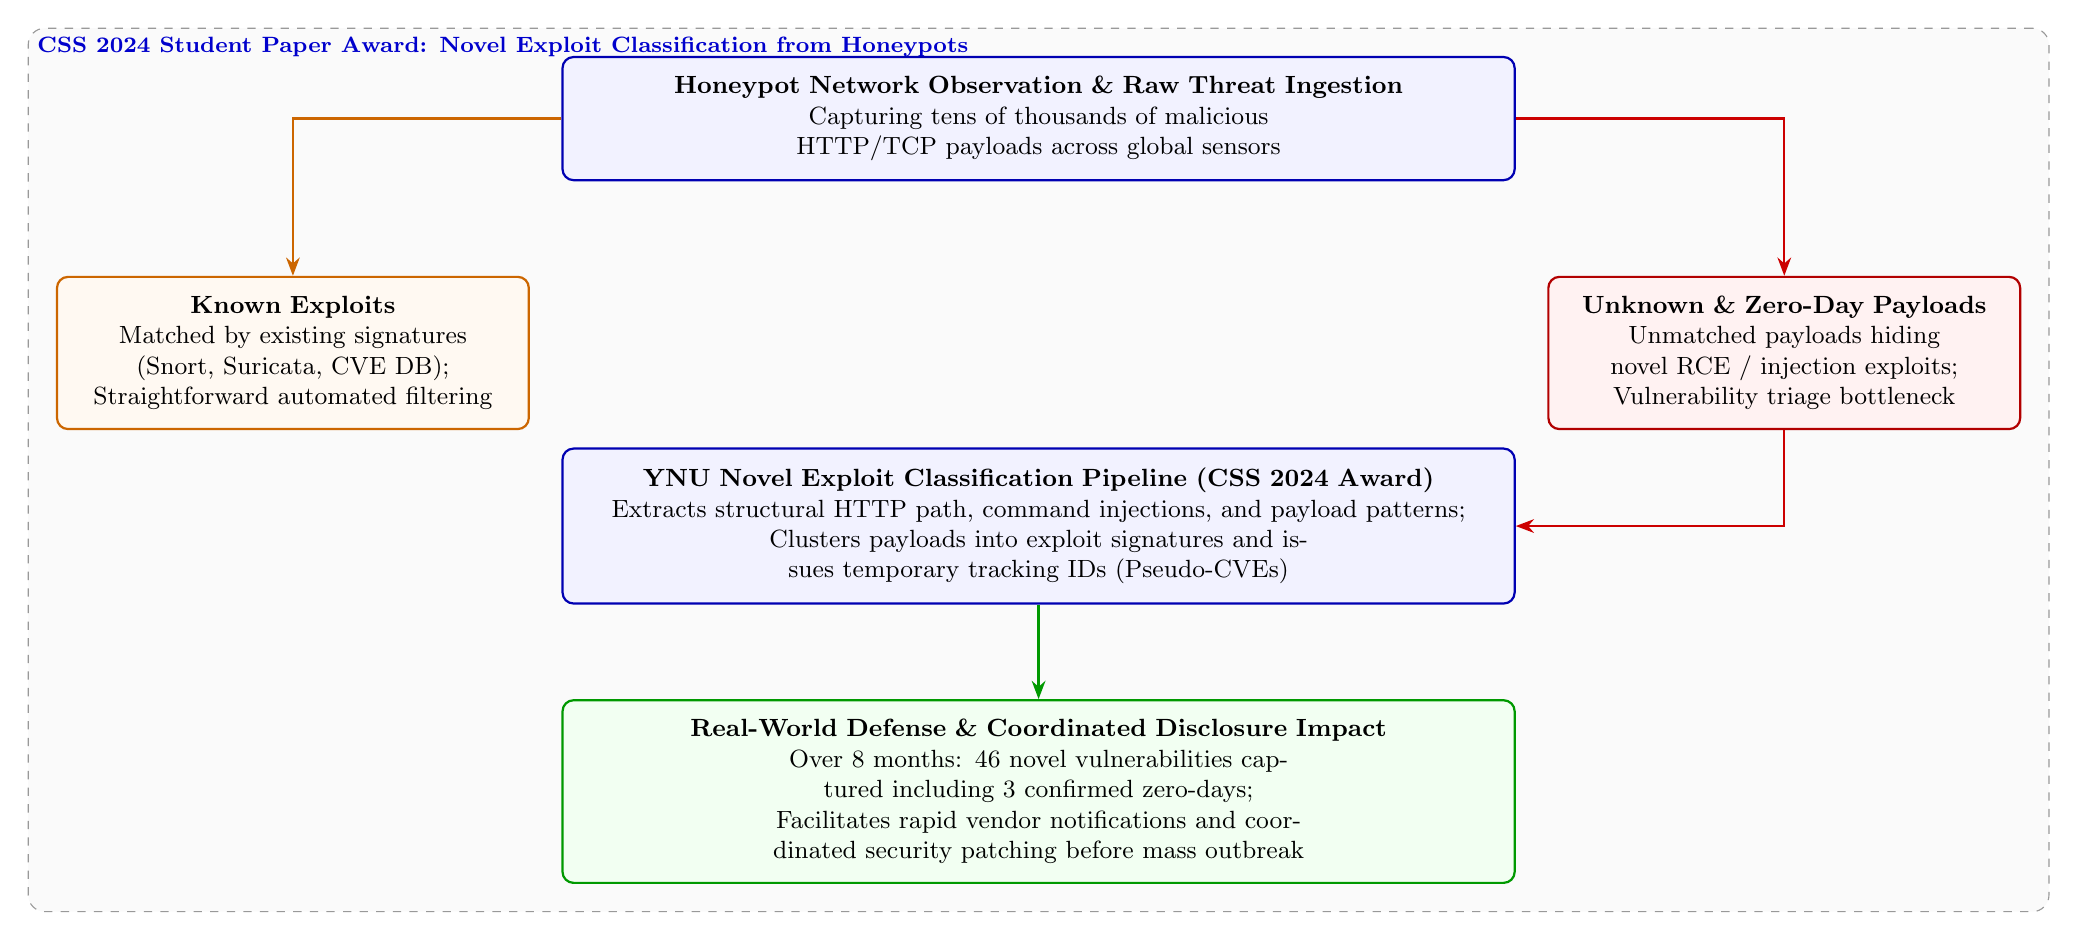
\begin{tikzpicture}[
    font=\small,
    >=Stealth,
    node distance=1.2cm,
    block/.style={rectangle, draw=blue!70!black, fill=blue!5, rounded corners=4pt, thick, align=center, inner sep=7pt},
    alertblock/.style={rectangle, draw=red!70!black, fill=red!5, rounded corners=4pt, thick, align=center, inner sep=7pt},
    greenblock/.style={rectangle, draw=green!60!black, fill=green!5, rounded corners=4pt, thick, align=center, inner sep=7pt},
    amberblock/.style={rectangle, draw=orange!80!black, fill=orange!5, rounded corners=4pt, thick, align=center, inner sep=7pt},
    groupbox/.style={draw=black!40, dashed, rounded corners=6pt, fill=black!2, inner sep=10pt}
]

    % Top: Honeypot Observation
    \node[block, text width=11.6cm] (honeypot) {\textbf{Honeypot Network Observation \& Raw Threat Ingestion}\\Capturing tens of thousands of malicious HTTP/TCP payloads across global sensors};

    % Left: Known vs Unknown
    \node[amberblock, below left=1.2cm and 0.4cm of honeypot, text width=5.5cm] (known) {\textbf{Known Exploits}\\Matched by existing signatures (Snort, Suricata, CVE DB);\\Straightforward automated filtering};

    \node[alertblock, below right=1.2cm and 0.4cm of honeypot, text width=5.5cm] (unknown) {\textbf{Unknown \& Zero-Day Payloads}\\Unmatched payloads hiding novel RCE / injection exploits;\\Vulnerability triage bottleneck};

    \draw[->, thick, orange!80!black] (honeypot) -| (known);
    \draw[->, thick, red!80!black] (honeypot) -| (unknown);

    % Middle: Novel Clustering & Signature Generation
    \node[block, below=1.2cm of $(known)!0.5!(unknown)$, text width=11.6cm] (clustering) {\textbf{YNU Novel Exploit Classification Pipeline (CSS 2024 Award)}\\Extracts structural HTTP path, command injections, and payload patterns;\\Clusters payloads into exploit signatures and issues temporary tracking IDs (Pseudo-CVEs)};

    \draw[->, thick, red!80!black] (unknown) |- (clustering);

    % Bottom: Impact
    \node[greenblock, below=1.2cm of clustering, text width=11.6cm] (impact) {\textbf{Real-World Defense \& Coordinated Disclosure Impact}\\Over 8 months: 46 novel vulnerabilities captured including 3 confirmed zero-days;\\Facilitates rapid vendor notifications and coordinated security patching before mass outbreak};

    \draw[->, thick, green!60!black] (clustering) -- (impact);

    \begin{scope}[on background layer]
        \node[groupbox, fit=(honeypot) (known) (unknown) (clustering) (impact), label={[anchor=north west, font=\footnotesize\bfseries, blue!80!black]north west:CSS 2024 Student Paper Award: Novel Exploit Classification from Honeypots}] {};
    \end{scope}

\end{tikzpicture}
\end{document}
